Quand il ne se fige pas, le code suivant donne la \textit{\og période \fg} d'un naturel auquel on applique le procédé présenté dans la section \ref{conjecture}.

\begin{rawcode}
n     = 20181209
nmemo = n

results = []

while n not in results:
    results.append(n)
    n = sum(int(d)**2 for d in str(n))

print(f"{nmemo} a la période suivante :")
print(results[results.index(n):])

print()

before = results[:results.index(n)]

if before:
    print("Avant la 1ère période nous avons :")
    print(before)
else:
    print("On commence directement par la période.")
\end{rawcode}

\medskip

Le code précédent, où \verb+n = 20181209+, nous affiche :

\begin{rawcode}
20181209 a la période suivante :
[16, 37, 58, 89, 145, 42, 20, 4]

Avant la 1ère période nous avons :
[20181209, 155, 51, 26, 40]
\end{rawcode}


\medskip

\begin{figure}[t]
	\centering
	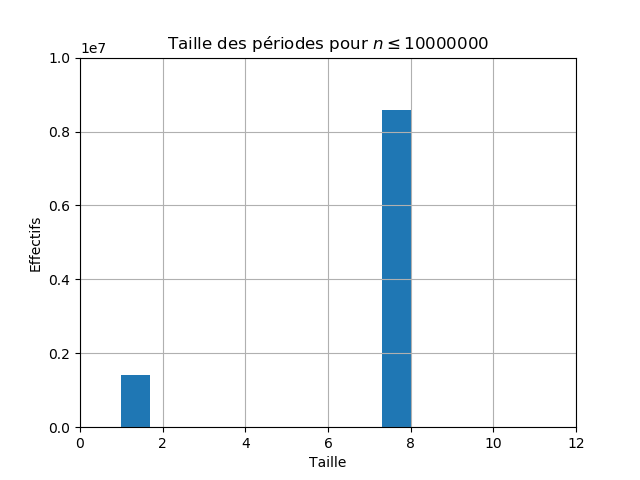
\includegraphics[scale=.9]{squares-digits/periods.png}
  	\caption{Histogramme des tailles des périodes}
	\label{histogram}
\end{figure}



\medskip

Amusons-nous maintenant à représenter un histogramme des tailles des \og périodes \fg{}
À l'adresse \url{https://github.com/bc-writing/drafts}, dans le dossier \texttt{squares-digits}, vous trouverez le fichier \texttt{squareint-sizeplots.py} qui été utilisé pour obtenir le graphique
\footnote{
	À la même adresse dans le dossier \texttt{squares-digits} se trouve l'image \texttt{befores.png} qui est un histogramme des nombres de termes calculés avant l'apparition de la 1\iere{} \emph{\og période \fg{}}.
}.
Le traitement des données a été amélioré pour éviter de refaire des calculs déjà rencontrés \emph{(pour plus de précisions, se reporter aux commentaires du code)}.
Le résultat est donné dans la figure \ref{histogram} \cpageref{histogram}.



\medskip

Le graphique est frappant ! En effet, il semblerait que l'on ait soit des périodes de taille $1$, penser à $0$ et $1$, soit des périodes de taille $8$ comme pour $37 - 58 - 89 - 145 - 42 - 20 - 4 - 16$.
Magie ou coïncidence ? Les résultats de la section \ref{proof}, dont nous allons reprendre les notations, vont nous permettre de le savoir.
Tout d'abord,  d'après le fait \ref{magicmajo}, nous avons $\taille(sq(n)) < \taille(n)$ dès que $\taille(n) \geqslant 4$, donc la périodicité n'arrivera que lorsque $\taille\left( \, \sqseq{n}{k} \right) \leqslant 3$.
De plus, nous savons aussi que $\taille(sq(n)) \leqslant 3$ dès que $\taille(n) \leqslant 3$.
Tout ceci nous permet d'analyser brutalement via un programme ce qu'il se passe pour les périodes des naturels appartenant à $\ZintervalC{0}{999}$. Nous pouvons pour cela utiliser le code suivant, qui n'est absolument pas optimisé mais fait le travail immédiatement.


\newpage

\begin{rawcode}
nmax = 999

periodsfound = []

for n in range(nmax + 1):
    results = []

    while n not in results:
        results.append(n)
        n = sum(int(d)**2 for d in str(n))

    period = results[results.index(n):]

    if period not in periodsfound:
        periodsfound.append(period)

for oneperiod in periodsfound:
    print(oneperiod)
\end{rawcode}



\medskip

Le code précédent nous fournit toutes les périodes possibles.


\newpage

\begin{rawcode}
[0]
[1]
[4, 16, 37, 58, 89, 145, 42, 20]
[37, 58, 89, 145, 42, 20, 4, 16]
[89, 145, 42, 20, 4, 16, 37, 58]
[16, 37, 58, 89, 145, 42, 20, 4]
[20, 4, 16, 37, 58, 89, 145, 42]
[58, 89, 145, 42, 20, 4, 16, 37]
[42, 20, 4, 16, 37, 58, 89, 145]
[145, 42, 20, 4, 16, 37, 58, 89]
\end{rawcode}


\medskip

Et là cela devient joli car nous notons au passage que trois types de périodes : 
\verb+[0]+, \verb+[1]+ et
\verb+[4, 16, 37, 58, 89, 145, 42, 20]+ avec toutes ses \emph{\og permutées circulaires \fg}.